\chapter[Time Series with Constant Variance]{Time Series with Constant Variance (10\% à 20\%)}

\subsection{Information}

\begin{distributions}[Description]
Notes du descriptif principal:
\begin{itemize}
	\item	Covers an introduction to modeling activity, such as financial results or stock prices, over time;
	\item	The model used is the Auto Regressive Integrated Moving Average (ARIMA) where activity in a given period may be linked to activity in subsequent time periods;
	\item	The connection between adjacent time periods violates one of the assumptions behind the Extended Linear Model techniques;
	\item	The ARIMA appproach incorporates that linkage as an aid for it's predictions;
	\item	Also covers the application of regression models to time series analysis;
\end{itemize}
\tcbline
Notes de la sous-section:
\begin{itemize}
	\item	Section covers basic applications of the ARIMA time series model;
\end{itemize}
\end{distributions}

\begin{outcomes}[Learning objectives]
\begin{enumerate}
	\item	Use time series to model trends;
		\begin{itemize}
		\item	Estimation, data analysis, and forecasting;
		\item	Forecast errors and confidence intervals;
		\end{itemize}
	\begin{knowledge}[Knowledge Statements]
	\begin{enumerate}
	\item	Mean-reverting time series;
	\item	Elimination of trends using differencing;
	\item	Relationship between seasonality and autocorrelation;
	\end{enumerate}
	\end{knowledge}
\tcbline
	\item	Model relationships of current and past values of a statistic / metric;
		\begin{itemize}
		\item	Estimation, data analysis, and forecasting;
		\item	Forecast errors and confidence intervals;
		\end{itemize}
	\begin{knowledge}[Knowledge Statements]
	\begin{enumerate}
	\item	Calculation and use of lag $k$ autocorrelation statistic and cross correlation statistics in determining model structure;
	\item	Stationary series;
	\item	AR(1) models;
	\item	ARIMA models---AR(p), MA(q), ARMA(p, q), ARIMA(p, d, q), ARMA vs ARIMA;
	\item	Invertible time series and relationship between AR and MA models;
	\item	Converting between AR and MA models;
	\item	Interpretation of auto-correlation function as aid to model selection (AR vs. MA and number of lags to include in model);
	\item	Relationship between time series input and item modeled for AR vs. MA;
	\end{enumerate}
	\end{knowledge}
\tcbline
	\item	Understand forecasts produced by ARIMA;
	\begin{knowledge}[Knowledge Statements]
	\begin{enumerate}
	\item	Forecast using ARIMA models;
	\item	\textbf{One} step ahead \textit{prediction} vs \textbf{many} step ahead \textit{projection};
	\item	Change in variance in prediction by AR vs MA model;
	\end{enumerate}
	\end{knowledge}
\tcbline
	\item	Time Series with Regression;
	\begin{knowledge}[Knowledge Statements]
	\begin{enumerate}
	\item	Deterministic vs. Stochastic Trend;
	\item	Serial correlation in regression error results;
	\item	Correction in regression via Generalized Least Squares;
	\item	Transformation of data using natural logarithms for regression modelling;
	\item	Forecast error correction under natural logarithms transformation;
	\end{enumerate}
	\end{knowledge}
\end{enumerate}
\end{outcomes}

\begin{ASM_chapter}[Related lessons ASM]
\begin{itemize}
	\item[]	\nameref{L.-57}
	\item[]	\nameref{L.-58}
	\item[]	\nameref{L.-59}
	\item[]	\nameref{L.-60}
	\item[]	\nameref{L.-61}
	\item[]	\nameref{L.-62}
	\item[]	\nameref{L.-63}
	\item[]	\nameref{L.-64}
\end{itemize}
\end{ASM_chapter}

\begin{YTB_vids}[Vidéos YouTube]
\begin{itemize}
	\item	
\end{itemize}
\end{YTB_vids}

\subsection{Résumés des chapitres}

\begin{CHPT_SUMM_AUTO}[label = {L.-57}]{57. Time Series: Trend and Seasonality}
Introduction to Time Series with \texttt{R} 1
\begin{itemize}
	\item[1.1:]	Time Series Data---Purpose;
		\begin{itemize}
		\item	Understand the past and predict the future;
		\item	Usage by Singapore Airlines to increase their fleet based on future goals (expansion) and past trends (growing popularity);
		\item	Usage by gas suppliers in the UK who must purchase the supply the day before it's demanded from offshore fields;
		\item[]	The price thus varies according to the temperature, the time of year, etc. and even the wind temperature.
		\end{itemize}
	\item[1.2:]	Time Series Data---Time Series;
		\begin{itemize}
		\item	Idea that variables are measured sequentially in time everywhere;
		\item[]	Banks record interest and exchange rates on a daily basis;
		\item[]	Governments measure GDP on a yearly basis;
		\item	Time series model, a.k.a. \textbf{discrete-time stochastic process}, is a \textbf{sequence} of \textit{random variables} defined at \textbf{fixed} \textbf{sampling intervals};
		\item	Main \textbf{features} of time series are \textbf{trends} and \textbf{seasonal variations};
		\item	Another important feature is that most observations which are close together in time tend to be correlated \textit{(serially dependent)};
		\item	This can be applied to making predictions and test whether, for example, fluctuations in sales are due to an underlying change or just regular variation;
		\item	Sampling intervals can differ in their relation to data.
			\begin{itemize}
			\item	The data could have been aggregated over the period (for example, the number of foreign tourists arriving per day);
			\item	The data could have been sampled over the period (for example, the daily close price of Apple stock).
			\end{itemize}
		\end{itemize}
	\item[1.3:]	Time Series Data---\texttt{R language};
	\item[1.4:]	Time Series Data---Plots, trends, and seasonal variation;
		\begin{itemize}
		\item	\textbf{Trend}: systemic change in a time series which doesn't appear to be periodic;
		\item[]	The simplest model for trends is a linear (de)increase and is often an adequate approximation;
		\item	\textbf{Seasonal variation}: Repeating pattern within each year;
		\item[]	For example, restaurant bookings varying according to the weekday;
		\item	\textbf{Cycles}: do not correspond to some \textbf{fixed} natural period
		\item[]	For example, the economic cycle;
		\item[]	\textit{No cycles are apparent in the image below:}
		
		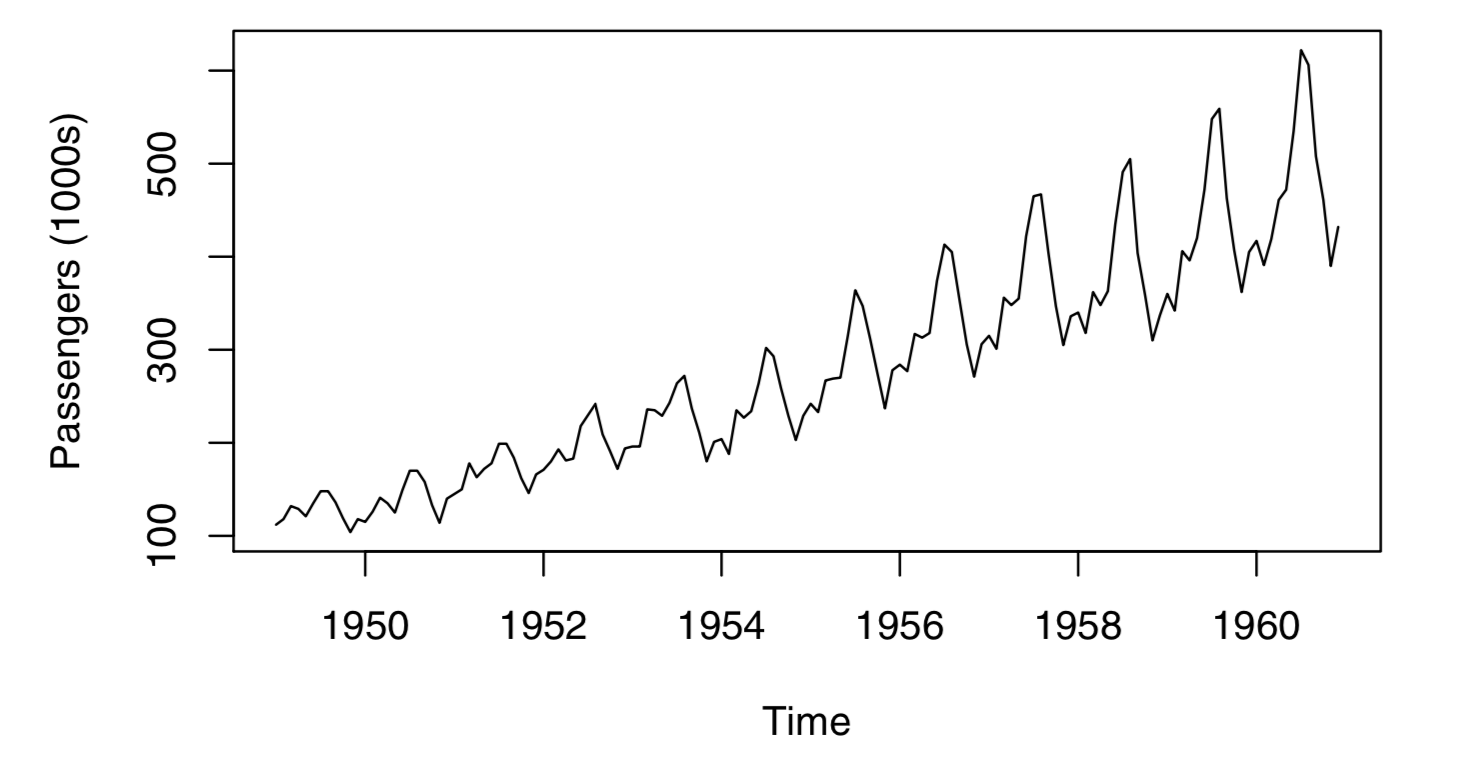
\includegraphics[scale=0.35]{src/TS-TREND.png}
		\item	The trend has many possible explanations (post-WWII prosperity, cheaper flights, etc.) but if there are non then it would be a \textbf{stochastic trend};
		\item[]	In this case, regression's not appropriate;
		\item	Forecasting uses extrapolation supposing trends continue at a slow pace;
		\item	Therefore, linear extrapolation is a reasonable approximation for a \textbf{few steps} ahead;
		\item[]	There's no empirical way to verify this, so we must explain the trend to justify extrapolation;
		\item	Forecasts beyond a year are thus better described as \textit{\textbf{scenarios}};
		\item	\textbf{Seasonal effects} can be \textit{removed} by \textit{aggregating to an annual basis} and evaluating the resulting time series;
		\item	Example of Chocolate/Beer/Electricity in Australia for \textit{Multiple Time Series};
		\item	Because autocorrelated series will often have the same trends and seasonal variations, they're often removed before comparison;
		\item	These trends will often be \textit{deterministic}
		\item[]	Australian population increase leads to an increase in electricity usage;
		\item	In contrast, finance will often have \textit{stochastic} trends;
		\item	Sometimes these can be modeled with a \textbf{random walk};
		\item	Idea of there being two distinct trends
		
		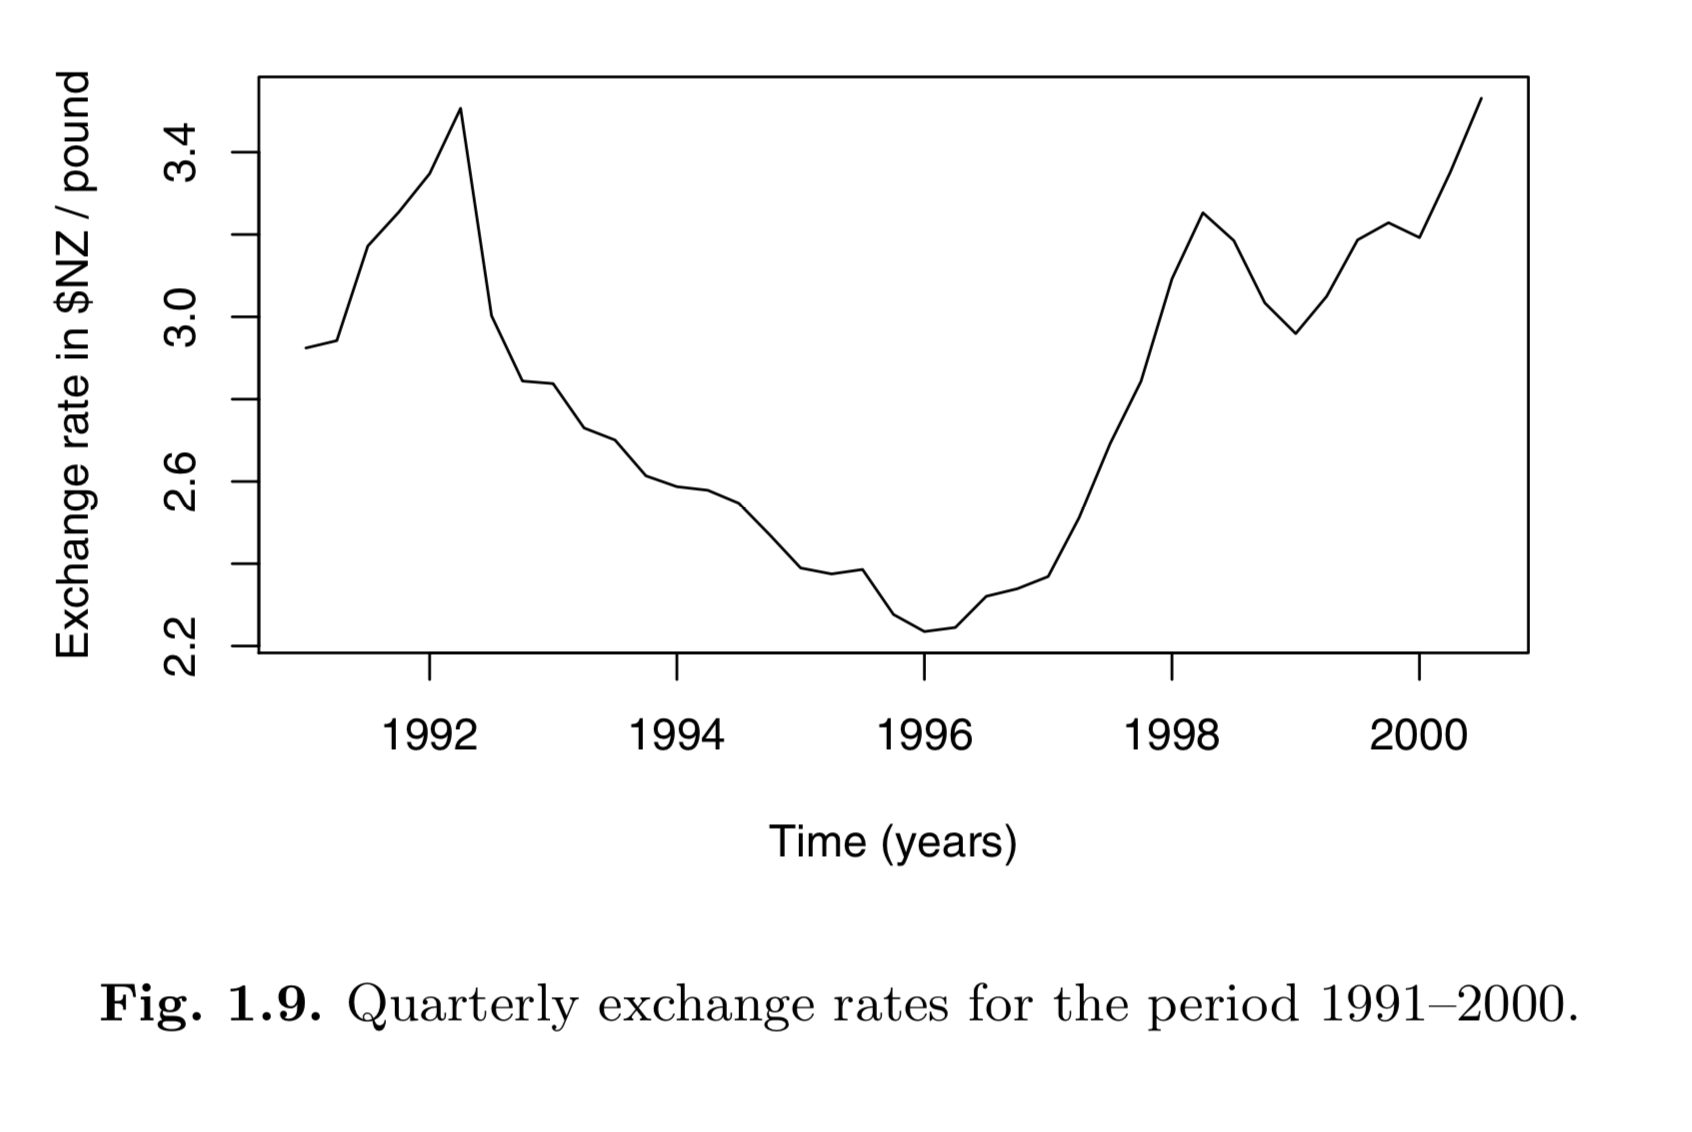
\includegraphics[scale=0.35]{src/TS-TREND-SPLIT.png}
		\item	Thereby, split the series in 2 (\texttt{window} in \texttt{R});
		
		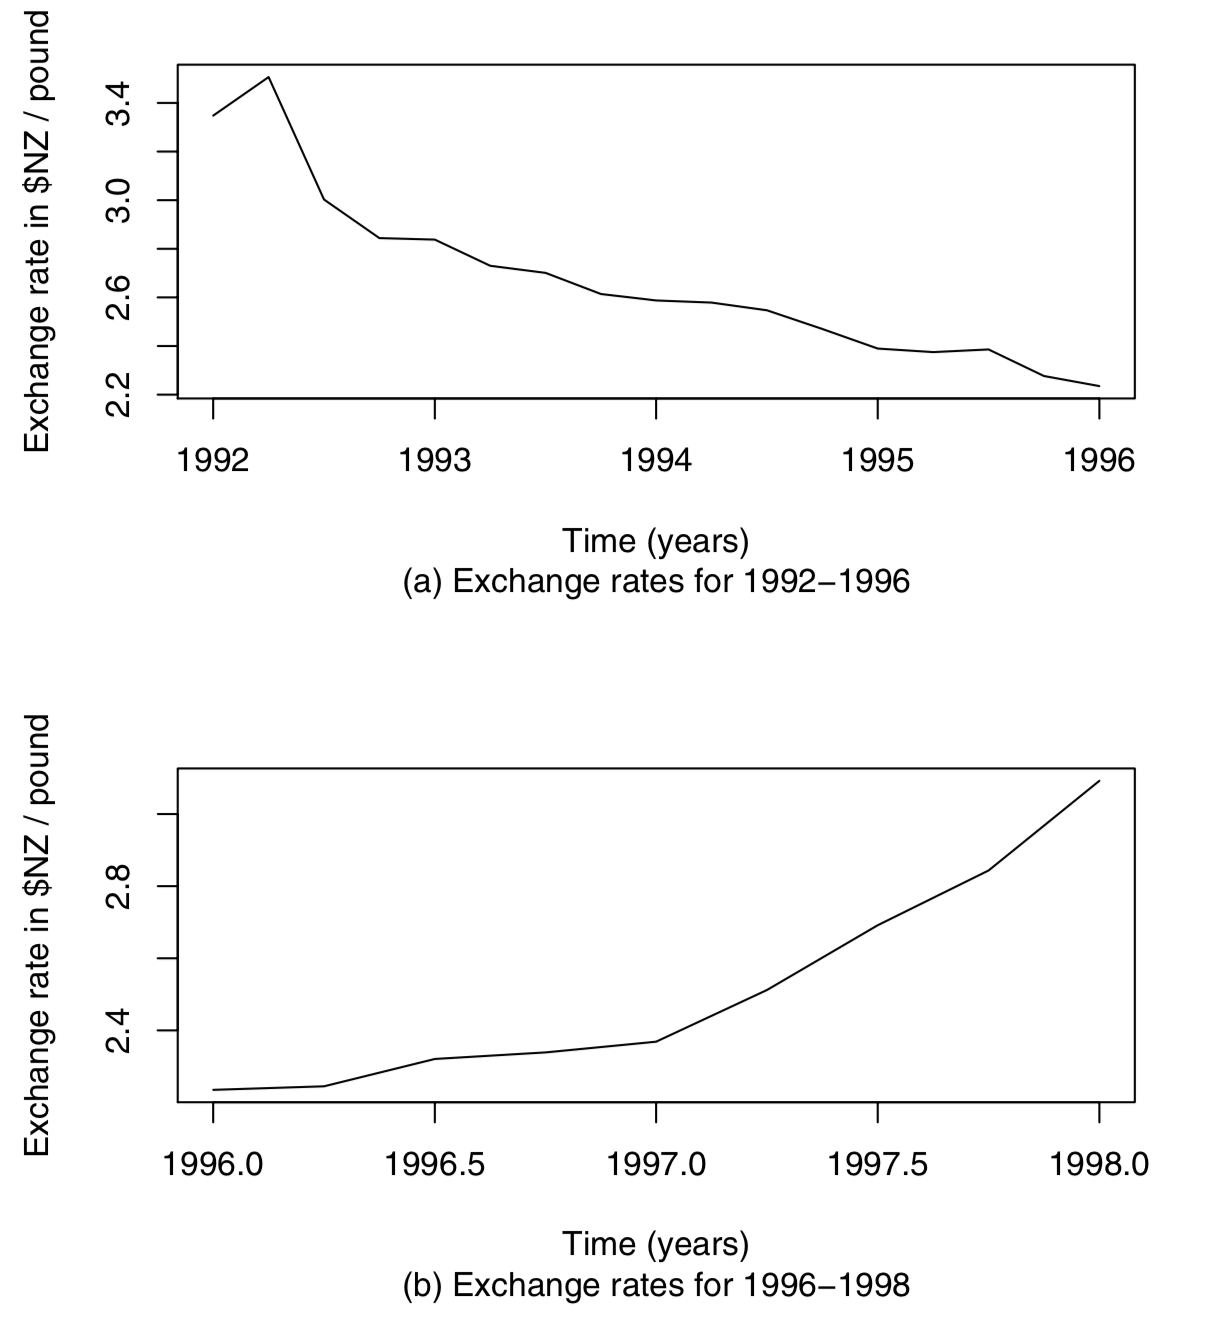
\includegraphics[scale=0.35]{src/TS-TREND-SPLIT-PLOTS.png}
		\item	This also highlights the importance of not extrapolating---without additional information we don't know whether the trend will continue;
		\item	Idea that 2 unrelated time series will be correlated if they both contain a trend thus we can't attribute global warming to fossil fuel increase without a physical explanation;
		\item	As per scientists, we judge appropriate to attribute a \textbf{causal relationship} and to expect mean global temperature to continue rising if greenhouse gas emissions aren't reduced;
		\end{itemize}
	\item[1.5:]	Time Series Data---Decomposition of series;
		\begin{itemize}
	\item	Time series of length $n$: $\{x_{t} : t = 1, \dots, n\} = \{x_{1}, x_{2}, \dots, x_{n}\}$;
	\item[]	It is a sequence of random variables $x_{t}$ sampled at $n$ discrete times $1, 2, \dots, n$;
	\item	Forecast at time $t$ for a future value $t + k$: $\hat{x}_{t + k | t}$;
	\item[]	$k$ is the \textbf{lead time};
		\end{itemize}
		\begin{itemize}
		\item	If the seasonal effect tends to increase as the trend increases, a multiplicative model may be more appropriate;
		\item	If there's a multiplicative factor modelled with the random variable (for example we have really large numbers) then an additive decomposition model for $\log(x_{t})$ may be more appropriate;
		\end{itemize}
		\begin{itemize}
		\item	Moving average centered around $x_{t}$ is one of the simplest ways to estimate a trend;
		\item[]	Because the average time is $t = 6.5$ and we have integer values, we have one half of both $x_{t - 6}$ and $x_{t + 6}$;
		\item	We can estimate the seasonal effect of each month $\bar{s}_{t}$ by averaging $\hat{s}_{t}$ per month;
		\item	We can take the mean of the averages and substract it from the time series and obtain the \textbf{seasonally adjusted series};
		\end{itemize}
		\begin{itemize}
		\item	\textbf{loess}: locally weighted regression technique;
		\item[]	\og \textit{local} \fg{} as it uses a \og small \fg{}  number of points \og around \fg{}  it;
		\item[]	Thereby, this reduces the impact of outliers;
		\end{itemize}
\end{itemize}

\begin{FORMULA_SUMM}{Formules chapitre 1}
Notation:
	\begin{align*}
	\text{time series}&:	
		\{x_{t} : t = 1, \dots, n\} 
	= 	\{x_{1}, x_{2}, \dots, x_{n}\}	\\
	\text{forecast}	&:	
		\hat{x}_{t + k | t}
	\end{align*}
	
Models
	\begin{align*}
	\text{additive decomposition model}	:	
	x_{t}	
	&=	m_{t} + s_{t} + z_{t}		\\
	\text{multiplicative model}	:	
	x_{t}	
	&=	m_{t} \cdot s_{t} + z_{t}		\\
	\text{additive decomposition model for }\log(x_{t})	:	
	x_{t}	
	&=	m_{t} + s_{t} + z_{t}	\\
	\text{forecast when }z_{t} \sim \mathcal{N}(0, \sigma^{2})	:
	\hat{x}_{t}	
	&=	\text{e}^{m_{t} + s_{t}}\text{e}^{\frac{1}{2}\sigma^{2}}
	\end{align*}
où
	\begin{multicols*}{2}
	\begin{description}
	\item[$x_{t}$]	observed series;
	\item[$m_{t}$]	trend;
	\item[$s_{t}$]	seasonal effect;
	\item[$z_{t}$]	error term.
	\end{description}
	\end{multicols*}
$z_{t}$ is generally a sequence of random variables with a mean of zero;

Moving average of a monthly series
	\setlength{\mathindent}{-1cm}
	\begin{align*}
	\hat{m}_{t}
	&=	\frac{\frac{1}{2} x_{t - 6} + x_{t - 5} + \dots + x_{t} + \dots + x_{t + 5} + x_{t + 6}}{12}	\\
	\end{align*}
	\setlength{\mathindent}{1cm}

	
Monthly additive effect:
	\begin{align*}
	\hat{s}_{t} 
	&= 	x_{t} - \hat{m}_{t}	\\
	\end{align*}
Adjustment such that $\bar{s} = 0$.
	
Monthly multiplicative effect:
	\begin{align*}
	\hat{s}_{t} 
	&= 	\frac{x_{t}}{\hat{m}_{t}}	\\
	\end{align*}
Adjustment such that $\bar{s} = 1$.


$\bar{s} = \frac{\sum_{t = 1}^{t = m}\hat{s}_{t}}{m}$.
Seasonally adjusted data: $x_{t} - \hat{s}_{t}$.
\end{FORMULA_SUMM}
\tcbline
%	\begin{itemize}
%		\item	
%	\end{itemize}
\end{CHPT_SUMM_AUTO}

\begin{CHPT_SUMM_AUTO}[label = {L.-58}]{58. Time Series: Correlation}
Introduction to Time Series with \texttt{R} 2 - 3.1
\begin{itemize}
	\item[2:]	Correlation
	\item[3.1:]	Forecasting Strategies---Purpose
\end{itemize}
\tcbline
	\begin{enumerate}
		\item	Second order properties of a time series;
		\item	Relationships of different time series;
	\end{enumerate}
\end{CHPT_SUMM_AUTO}

\begin{CHPT_SUMM_AUTO}[label = {L.-59}]{59. Time Series: White Noise and Random Walks}
Introduction to Time Series with \texttt{R} 4.1 - 4.4
\begin{itemize}
	\item[4.1:]	Basic Stochastic Models---Purpose
	\item[4.2:]	Basic Stochastic Models---White Noise
	\item[4.3:]	Basic Stochastic Models---Random Walks
	\item[4.4:]	Basic Stochastic Models---Fitted models and diagnostic plots
\end{itemize}
\tcbline
	\begin{enumerate}
		\item	White noise;
		\item	Random walks;
	\end{enumerate}
\end{CHPT_SUMM_AUTO}

\begin{CHPT_SUMM_AUTO}[label = {L.-60}]{60. Time Series: Autoregressive Models}
Introduction to Time Series with \texttt{R} 4.5 - 4.8
\begin{itemize}
	\item[4.5:]	Basic Stochastic Models---AR models
	\item[4.6:]	Basic Stochastic Models---Fitted models
	\item[4.7:]	Basic Stochastic Models---Summary of \texttt{R} commands
	\item[4.8:]	Basic Stochastic Models---Exercices
\end{itemize}
\tcbline
	\begin{enumerate}
		\item[]	Correlograms and partial correlograms;
		\item[]	Stationnarity;
		\item[]	Forecasting with $AP(p)$ series;
	\end{enumerate}
\end{CHPT_SUMM_AUTO}

\begin{CHPT_SUMM_AUTO}[label = {L.-61}]{61. Time Series: Regression}
Introduction to Time Series with \texttt{R} 5
\begin{itemize}
	\item[5:]	Regression
\end{itemize}
\tcbline
	\begin{enumerate}
		\item	Correcting for autocorrelation;
		\item	Seasonality;
		\item	Logarithmic transformations;
		\item	Error correction factors;
	\end{enumerate}
\end{CHPT_SUMM_AUTO}

\begin{CHPT_SUMM_AUTO}[label = {L.-62}]{62. Time Series: Moving Average Models}
Introduction to Time Series with \texttt{R} 6.1 - 6.4
\begin{itemize}
	\item[6.1:]	Stationary Models---Purpose
	\item[6.2:]	Stationary Models---Strictly stationary series
	\item[6.3:]	Stationary Models---MA models
	\item[6.4:]	Stationary Models---Fitted MA models
\end{itemize}
\tcbline
	\begin{itemize}
		\item	
	\end{itemize}
\end{CHPT_SUMM_AUTO}

\begin{CHPT_SUMM_AUTO}[label = {L.-63}]{63. Time Series: ARMA Models}
Introduction to Time Series with \texttt{R} 6.5 - 6.8
\begin{itemize}
	\item[6.5:]	Stationary Models---Mixed models: The ARMA process
	\item[6.6:]	Stationary Models---ARMA models: Empirical Analysis
	\item[6.7:]	Stationary Models---Summary of \texttt{R} commands
	\item[6.8:]	Stationary Models---Exercices
\end{itemize}
\tcbline
	\begin{itemize}
		\item	
	\end{itemize}
\end{CHPT_SUMM_AUTO}

\begin{CHPT_SUMM_AUTO}[label = {L.-64}]{64. Time Series: ARIMA and SARIMA Models}
Introduction to Time Series with \texttt{R} 7.1 - 7.3
\begin{itemize}
	\item[7.1:]	Non-stationary Models---Purpose
	\item[7.2:]	Non-stationary Models---Non-Seasonal ARIMA models
	\item[7.3:]	Non-stationary Models---Seasonal ARIMA models
\end{itemize}
\tcbline
	\begin{itemize}
		\item	
	\end{itemize}
\end{CHPT_SUMM_AUTO}

\subsection{Notes sur les vidéos YouTube}

\begin{YTB_SUMM}[label = {SQ-BASICS-ML-INTRO}]{\href{https://www.youtube.com/watch?v=Gv9_4yMHFhI&list=PLblh5JKOoLUICTaGLRoHQDuF_7q2GfuJF&index=2&t=0s}{StatQuest: A Gentle Introduction to Machine Learning}}
\begin{itemize}
	\item	
\end{itemize}
\end{YTB_SUMM}